%% Figure C1. The chain on PHerc. 0826 as boxes, each the exact program and mode it runs.
%% The nodes and arrows are c-f1-pipeline-body.tex, generated by tools/c-f1-pipeline.py from the
%% rows of ../evidence/figures/c-f1-pipeline.csv; nothing is typed here but the styles. The third line of
%% each box is its measured factor (blue) or «not measured» (grey italic), from the same rows.
\documentclass[border=3pt]{standalone}
%% THIS FILE IS SHARED. Its one source is results/figpreamble.tex and the copy in each work's
%% src/tools is taken from it, because a published folder has to stand on its own and cannot
%% follow a link out of itself. tools/check_figpreamble.py refuses a copy that has drifted.
%%
%% It is one file because it was two, and they drifted: the panel title correction of
%% 2026-09-22T06:44Z was made in one work's copy and never reached the other, so that work drew
%% both panel titles at the axis origin, inside the plot and over the first bar, until
%% 2026-09-22T14:33Z. One source and a check is what stops that happening twice.

%% figpreamble.tex: what every figure of this work loads, and the one filter they all use.
%%
%% Every figure is a standalone pgfplots document that reads its numbers with pgfplotstable from
%% the CSV its own data script wrote under evidence/figures/. No number is typed in a figure
%% source. That is not a style: it is what makes the picture and the table of plotted numbers
%% unable to disagree, because they are the same file read twice.
%%
%% The CSVs written by tools/figlib.py open with one comment line, so every table is read with
%% skip first n=1, and they carry no comma inside a cell, so col sep=comma is exact.
\usepackage{pgfplots}
\usepackage{pgfplotstable}
\pgfplotsset{compat=1.18}
\usepgfplotslibrary{groupplots}

\pgfplotstableset{col sep=comma, skip first n=1, trim cells}

%% One CSV per figure, and no filtering in the figure source.
%%
%% The plotted tables are wide: one row per position on the abscissa, one column per series.
%% That is not a taste, it is what works. pgfplotstable parses every cell of a column an
%% \addplot names, and its read time row filter does not see column values, so a long table with
%% one row per series cannot be split inside the figure: the rows of the other series are parsed
%% too. The first render of figure S2 failed on exactly that, on the cell "not measurable", and
%% the tables were rewritten wide. A series with no value at a position carries nan, which
%% pgfplots drops with its default unbounded coords setting, and never a zero; the words the
%% study used sit in the status column beside the number.

%% One neutral set of marks and fills, light background, no colour carrying meaning on its own:
%% every series is also told apart by its mark, because a reader printing in grey is still a
%% reader.
\pgfplotsset{
  sa base/.style={
    width=82mm, height=58mm,
    tick align=outside, tick pos=left,
    grid=major, grid style={gray!25, very thin},
    axis line style={gray!60},
    label style={font=\small}, tick label style={font=\footnotesize},
    legend style={font=\footnotesize, draw=gray!50, fill=white, fill opacity=0.9,
                  text opacity=1, cells={anchor=west}},
    %% The title sits ABOVE the panel and not on it: with `above` alone it landed on the
    %% plot area and over the tick labels of the panel beside it, seen 2026-09-22T06:44Z.
    every axis title/.style={font=\small, at={(0.5,1)}, anchor=south, yshift=2.5mm},
  },
  %% A legend BELOW the panel, outside the plot area entirely, in one row.
  %%
  %% Written 2026-09-22 on the director's rejection of figure S1. `sa base` gives the legend
  %% `fill opacity=0.9`, so a legend placed inside does not hide what is under it, it GHOSTS it:
  %% on S1 the legend sat over the seed40 pair and its «200 times» label showed through the box
  %% as pale grey text, which is worse than hiding it, because a reader sees something is there
  %% and cannot read it. The remedy is not a better corner. A legend inside the plot area has to
  %% be re placed by hand every time the data moves, and nobody checks. Outside, it cannot
  %% collide with anything at any data value.
  %%
  %% The negative y in `at` is in axis fractions, so it follows `height` and does not have to be
  %% retuned. 0.32 clears rotated tick labels at \tiny; a panel with longer ones passes its own.
  sa legend below/.style={
    legend style={at={(0.5,-0.32)}, anchor=north, legend columns=-1,
                  font=\footnotesize, draw=gray!50, fill=white, fill opacity=1,
                  text opacity=1, cells={anchor=west},
                  /tikz/every even column/.append style={column sep=4mm}},
  },
  sa bars/.style={
    sa base, ybar, bar width=4pt, enlarge x limits=0.08,
  },
  sa stacked/.style={
    sa base, ybar stacked, bar width=14pt, enlarge x limits=0.28,
  },
}
\definecolor{sablue}{RGB}{31,78,121}
\definecolor{saorange}{RGB}{191,98,4}
\definecolor{sagrey}{RGB}{110,110,110}
\definecolor{sagreen}{RGB}{31,110,70}

%% ---- Addition of 2026-09-28T18:30Z (coordinator, director's note of 18:29:38Z, owner's word) ----
%% One visual language across S, A, the umbilicus and the PHerc. 0826 article: IEEE serif type and
%% one colour blind safe palette, the Okabe and Ito set (Okabe M., Ito K., Color Universal Design,
%% 2002, the eight colours of its table). The four names above keep their names and take Okabe Ito
%% values, so every figure that already uses them follows. Colours carry a ROLE, the umbilicus
%% work's rule: our result blue, the reference or the published label orange, an outcome we do not
%% want vermillion; a second series of ours sky blue, a third bluish green; neutral grey. The same
%% values, under the same role names, are in results/figstyle.py for the rasters and matplotlib.
\usepackage{mathptmx}
\definecolor{sablue}{RGB}{0,114,178}
\definecolor{saorange}{RGB}{230,159,0}
\definecolor{sagrey}{RGB}{110,110,110}
\definecolor{sagreen}{RGB}{0,158,115}
\definecolor{sasky}{RGB}{86,180,233}
\definecolor{savermillion}{RGB}{213,94,0}
\definecolor{sapurple}{RGB}{204,121,167}
\definecolor{sayellow}{RGB}{240,228,66}
\colorlet{saours}{sablue}
\colorlet{saref}{saorange}
\colorlet{sabad}{savermillion}
\pgfplotscreateplotcyclelist{sa roles}{
  {sablue, mark=*}, {saorange, mark=square*}, {sasky, mark=triangle*},
  {sagreen, mark=diamond*}, {savermillion, mark=pentagon*}, {sapurple, mark=o}, {sagrey, mark=x}}
\pgfplotsset{sa base/.append style={cycle list name=sa roles, axis x line*=bottom, axis y line*=left}}

\usetikzlibrary{arrows.meta}
\begin{document}
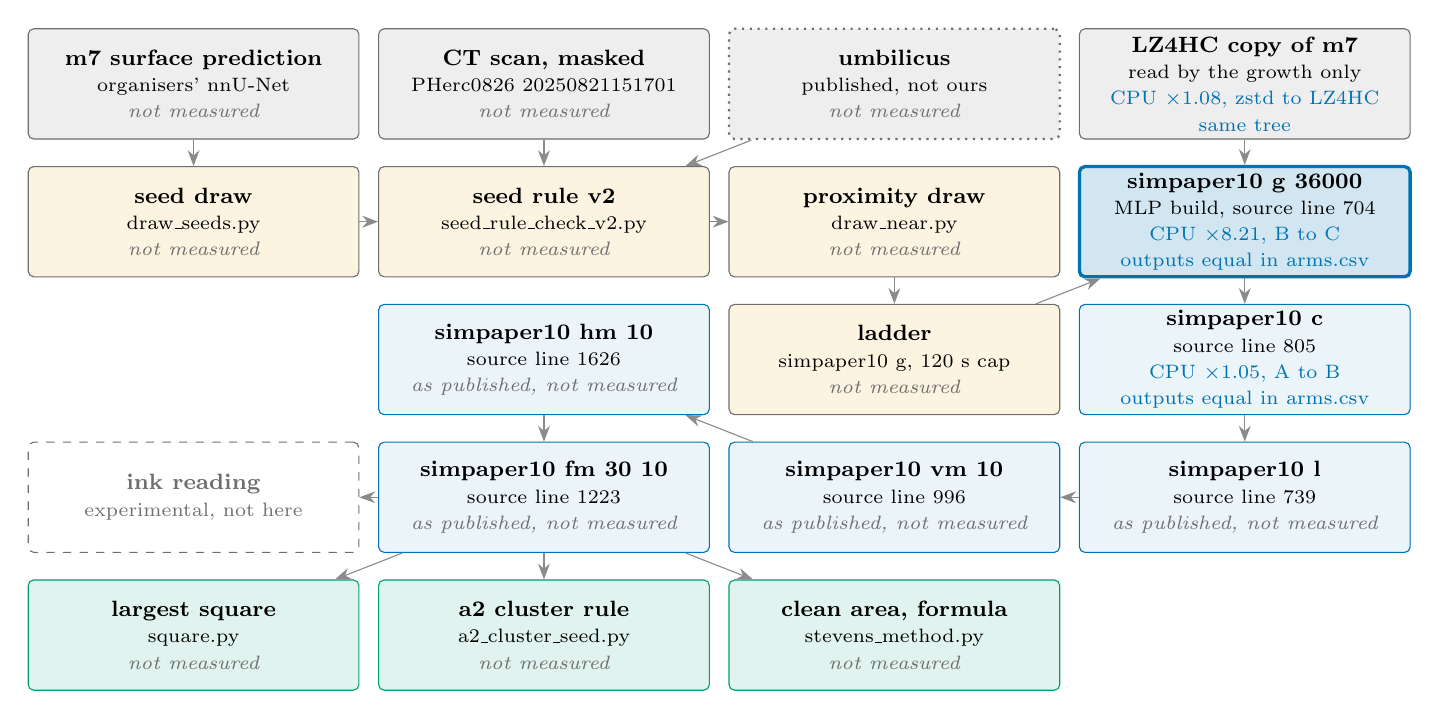
\begin{tikzpicture}[font=\footnotesize,
  box/.style={draw=sagrey, rounded corners=2pt, align=center, minimum width=42mm, minimum height=14mm, inner sep=2pt},
  data/.style={fill=sagrey!12},
  external/.style={fill=sagrey!12, dotted, thick},
  select/.style={fill=saorange!12},
  growth/.style={fill=sablue!18, very thick, draw=sablue},
  stage/.style={fill=sablue!8, draw=sablue},
  measure/.style={fill=sagreen!12, draw=sagreen},
  experimental/.style={dashed, draw=sagrey, text=sagrey},
  arr/.style={-{Stealth[length=2mm]}, draw=sagrey!80, thin}]
%% Generated by src/tools/c-f1-pipeline.py from evidence/figures/c-f1-pipeline.csv. Do not edit.
\node[box, data] (ct) at (4.45,0.00) {\textbf{CT scan, masked}\\{\scriptsize PHerc0826 20250821151701}\\{\scriptsize\itshape\color{sagrey} not measured}};
\node[box, data] (m7) at (0.00,0.00) {\textbf{m7 surface prediction}\\{\scriptsize organisers' nnU-Net}\\{\scriptsize\itshape\color{sagrey} not measured}};
\node[box, data] (lz) at (13.35,0.00) {\textbf{LZ4HC copy of m7}\\{\scriptsize read by the growth only}\\{\scriptsize\color{sablue}CPU $\times$1.08, zstd to LZ4HC}\\{\scriptsize\color{sablue}same tree}};
\node[box, external] (umb) at (8.90,0.00) {\textbf{umbilicus}\\{\scriptsize published, not ours}\\{\scriptsize\itshape\color{sagrey} not measured}};
\node[box, select] (draw) at (0.00,-1.75) {\textbf{seed draw}\\{\scriptsize draw\_seeds.py}\\{\scriptsize\itshape\color{sagrey} not measured}};
\node[box, select] (rule) at (4.45,-1.75) {\textbf{seed rule v2}\\{\scriptsize seed\_rule\_check\_v2.py}\\{\scriptsize\itshape\color{sagrey} not measured}};
\node[box, select] (near) at (8.90,-1.75) {\textbf{proximity draw}\\{\scriptsize draw\_near.py}\\{\scriptsize\itshape\color{sagrey} not measured}};
\node[box, select] (ladder) at (8.90,-3.50) {\textbf{ladder}\\{\scriptsize simpaper10 g, 120 s cap}\\{\scriptsize\itshape\color{sagrey} not measured}};
\node[box, growth] (g) at (13.35,-1.75) {\textbf{simpaper10 g 36000}\\{\scriptsize MLP build, source line 704}\\{\scriptsize\color{sablue}CPU $\times$8.21, B to C}\\{\scriptsize\color{sablue}outputs equal in arms.csv}};
\node[box, stage] (s0) at (13.35,-3.50) {\textbf{simpaper10 c}\\{\scriptsize source line 805}\\{\scriptsize\color{sablue}CPU $\times$1.05, A to B}\\{\scriptsize\color{sablue}outputs equal in arms.csv}};
\node[box, stage] (s1) at (13.35,-5.25) {\textbf{simpaper10 l}\\{\scriptsize source line 739}\\{\scriptsize\itshape\color{sagrey} as published, not measured}};
\node[box, stage] (s2) at (8.90,-5.25) {\textbf{simpaper10 vm 10}\\{\scriptsize source line 996}\\{\scriptsize\itshape\color{sagrey} as published, not measured}};
\node[box, stage] (s3) at (4.45,-3.50) {\textbf{simpaper10 hm 10}\\{\scriptsize source line 1626}\\{\scriptsize\itshape\color{sagrey} as published, not measured}};
\node[box, stage] (s4) at (4.45,-5.25) {\textbf{simpaper10 fm 30 10}\\{\scriptsize source line 1223}\\{\scriptsize\itshape\color{sagrey} as published, not measured}};
\node[box, measure] (sq) at (0.00,-7.00) {\textbf{largest square}\\{\scriptsize square.py}\\{\scriptsize\itshape\color{sagrey} not measured}};
\node[box, measure] (a2) at (4.45,-7.00) {\textbf{a2 cluster rule}\\{\scriptsize a2\_cluster\_seed.py}\\{\scriptsize\itshape\color{sagrey} not measured}};
\node[box, measure] (area) at (8.90,-7.00) {\textbf{clean area, formula}\\{\scriptsize stevens\_method.py}\\{\scriptsize\itshape\color{sagrey} not measured}};
\node[box, experimental] (ink) at (0.00,-5.25) {\textbf{ink reading}\\{\scriptsize experimental, not here}};
\draw[arr] (m7) -- (draw);
\draw[arr] (draw) -- (rule);
\draw[arr] (ct) -- (rule);
\draw[arr] (umb) -- (rule);
\draw[arr] (rule) -- (near);
\draw[arr] (near) -- (ladder);
\draw[arr] (lz) -- (g);
\draw[arr] (ladder) -- (g);
\draw[arr] (g) -- (s0);
\draw[arr] (s0) -- (s1);
\draw[arr] (s1) -- (s2);
\draw[arr] (s2) -- (s3);
\draw[arr] (s3) -- (s4);
\draw[arr] (s4) -- (sq);
\draw[arr] (s4) -- (a2);
\draw[arr] (s4) -- (area);
\draw[arr] (s4) -- (ink);

\end{tikzpicture}
\end{document}
